\section{Computational constraints and reproducibility}
\label{sec:jesper-compute}
\contributionauthor{Jesper Eggers}
The instantiated RUEHL and final networks contain 383,559 and 1,804,487
parameters, respectively. Parameter count alone does not determine deployment
cost because feature construction and survival searches also execute for
every action. We therefore time the complete callback on an Apple M4,
using CPU inference with one PyTorch thread per evaluator process.
Several evaluations run concurrently; these are local measurements without
exclusive processor access. Observer diagnostics execute outside the timed
callback, while the engine retains its actual timeout enforcement.

Across 266,007 callbacks, no timeout or timeout skip occurs. Against
rule-based opponents, the native policy's median, 95th-percentile, and
maximum observed latencies are 4.08, 7.61, and 101.07\,ms, respectively,
below the configured 500\,ms allowance on this machine. Random callbacks
omit feature construction and neural inference, so their latency compares
complete deployment costs rather than the isolated cost of action ranking.

Figure~\ref{fig:jesper-latency} reports pooled action quantiles, rather than
averages of per-episode percentiles. Its intervals resample whole episodes.
The evaluated default artifact,
\path{agent_code/final_agent/Ultra_Network_agent_saved_model_v2.pt}, has SHA-256 prefix \texttt{c268c3fcb5df3491}; the
complete hash, source hashes, checkpoint metadata, opponent definitions,
seeds, dependencies, and action records are retained in the experiment
manifests. Reproduction uses the project's source repository,
\url{https://github.com/ericgoldclub/bomberman_rl}, and the supplementary
evaluation scripts. Inference latency and elapsed training time quantify
different workloads; the local measurements also do not establish compliance
on the tournament's AMD processor.

\begin{figure}[!htbp]
\centering
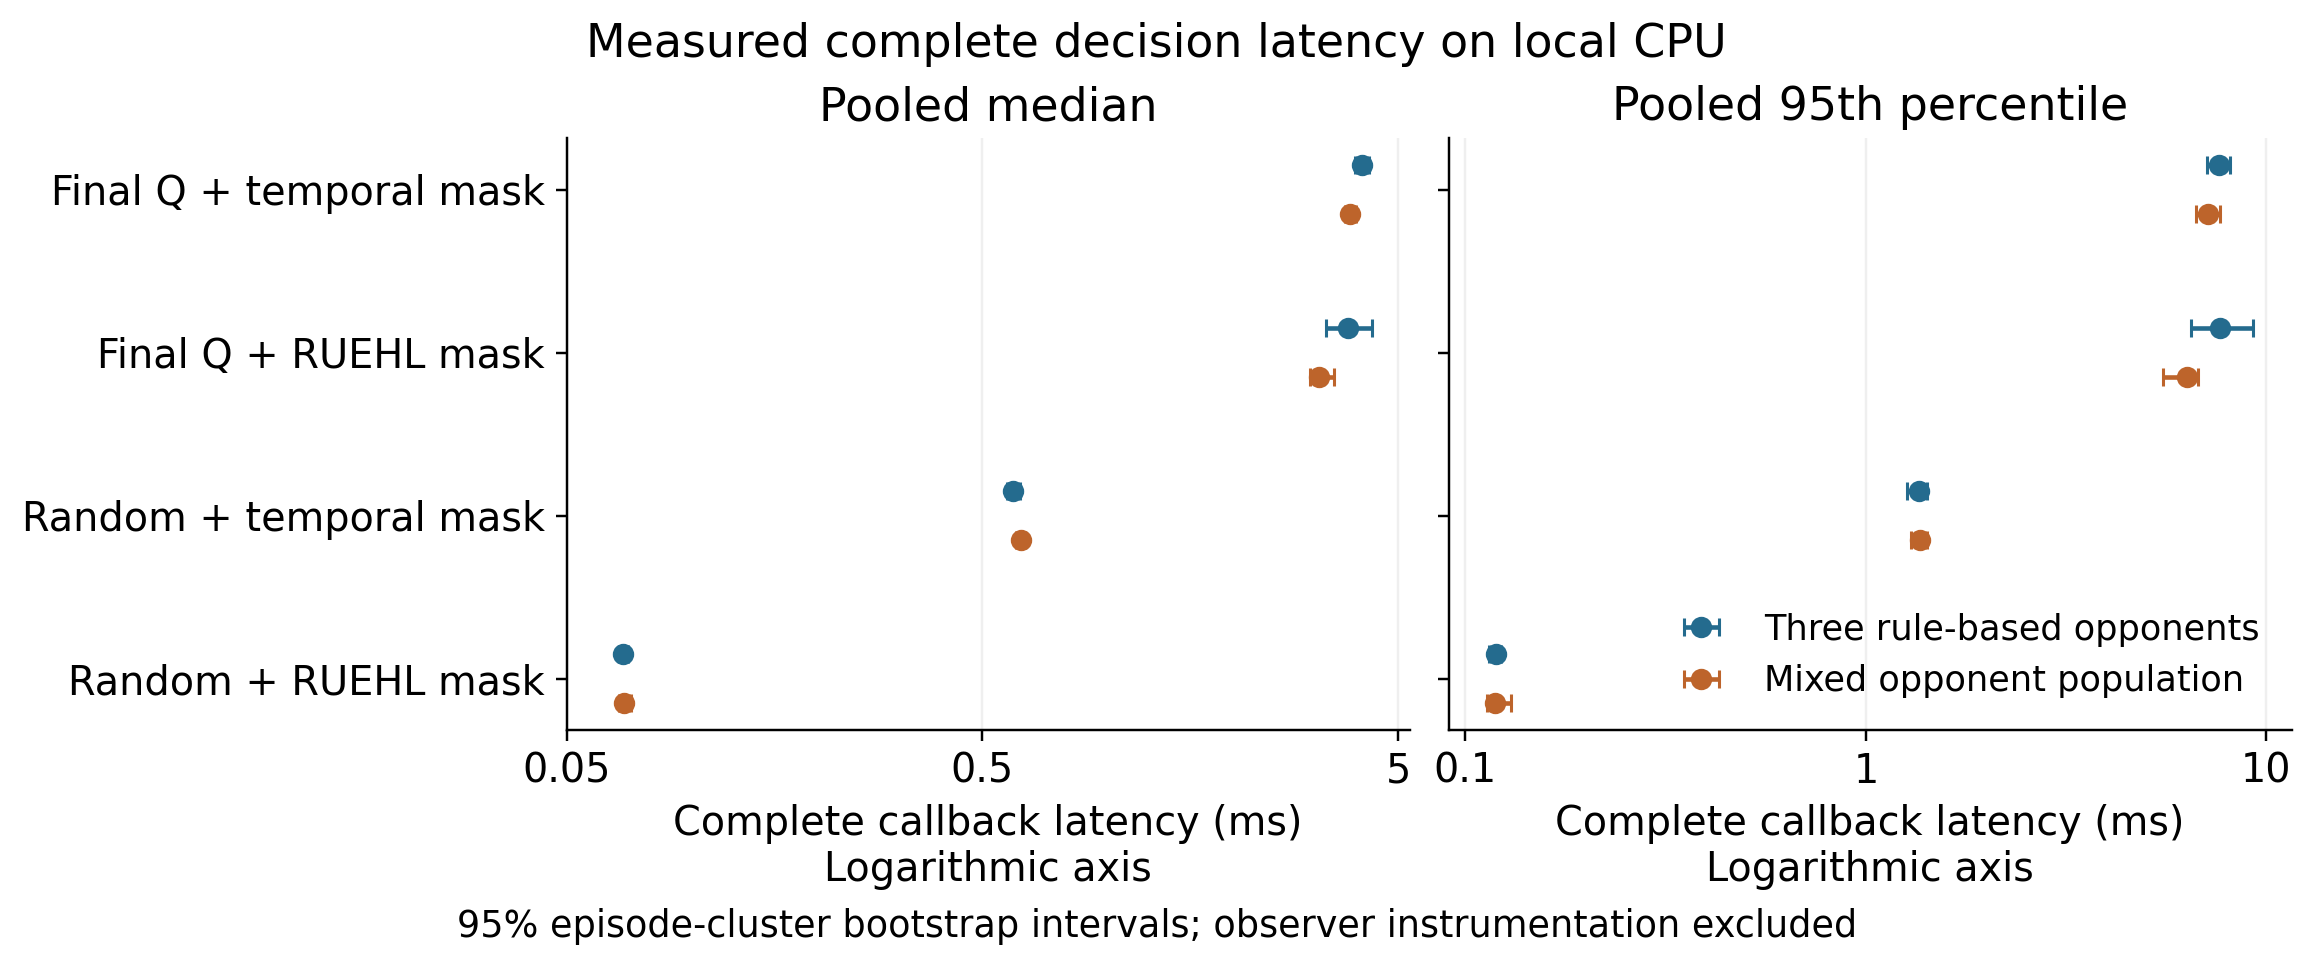
\includegraphics[width=\textwidth]{figures/frozen_evaluation_latency.png}
\caption{Complete callback latency. Learned rows include features, masking,
and network inference; random rows include masking and selection. Intervals
use 2,000 episode-cluster bootstrap
resamples. Concurrent local CPU evaluation does not reproduce the
tournament machine.}
\label{fig:jesper-latency}
\end{figure}
\FloatBarrier
